% Options for packages loaded elsewhere
\PassOptionsToPackage{unicode}{hyperref}
\PassOptionsToPackage{hyphens}{url}
\documentclass[
]{article}
\usepackage{xcolor}
\usepackage{amsmath,amssymb}
\setcounter{secnumdepth}{-\maxdimen} % remove section numbering
\usepackage{iftex}
\ifPDFTeX
  \usepackage[T1]{fontenc}
  \usepackage[utf8]{inputenc}
  \usepackage{textcomp} % provide euro and other symbols
\else % if luatex or xetex
  \usepackage{unicode-math} % this also loads fontspec
  \defaultfontfeatures{Scale=MatchLowercase}
  \defaultfontfeatures[\rmfamily]{Ligatures=TeX,Scale=1}
\fi
\usepackage{lmodern}
\ifPDFTeX\else
  % xetex/luatex font selection
\fi
% Use upquote if available, for straight quotes in verbatim environments
\IfFileExists{upquote.sty}{\usepackage{upquote}}{}
\IfFileExists{microtype.sty}{% use microtype if available
  \usepackage[]{microtype}
  \UseMicrotypeSet[protrusion]{basicmath} % disable protrusion for tt fonts
}{}
\makeatletter
\@ifundefined{KOMAClassName}{% if non-KOMA class
  \IfFileExists{parskip.sty}{%
    \usepackage{parskip}
  }{% else
    \setlength{\parindent}{0pt}
    \setlength{\parskip}{6pt plus 2pt minus 1pt}}
}{% if KOMA class
  \KOMAoptions{parskip=half}}
\makeatother
\usepackage{graphicx}
\makeatletter
\newsavebox\pandoc@box
\newcommand*\pandocbounded[1]{% scales image to fit in text height/width
  \sbox\pandoc@box{#1}%
  \Gscale@div\@tempa{\textheight}{\dimexpr\ht\pandoc@box+\dp\pandoc@box\relax}%
  \Gscale@div\@tempb{\linewidth}{\wd\pandoc@box}%
  \ifdim\@tempb\p@<\@tempa\p@\let\@tempa\@tempb\fi% select the smaller of both
  \ifdim\@tempa\p@<\p@\scalebox{\@tempa}{\usebox\pandoc@box}%
  \else\usebox{\pandoc@box}%
  \fi%
}
% Set default figure placement to htbp
\def\fps@figure{htbp}
\makeatother
\setlength{\emergencystretch}{3em} % prevent overfull lines
\providecommand{\tightlist}{%
  \setlength{\itemsep}{0pt}\setlength{\parskip}{0pt}}
\usepackage{bookmark}
\IfFileExists{xurl.sty}{\usepackage{xurl}}{} % add URL line breaks if available
\urlstyle{same}
\hypersetup{
  hidelinks,
  pdfcreator={LaTeX via pandoc}}

\author{}
\date{}

\begin{document}

{ATTENZIONE}

{I doppi - consecutivi dei comandi per via di come Google Documenti
gestisce i simboli sono mostrati come uno singolo, inoltre non è
consigliato copiare direttamente i comandi da qui sulla bash}

{}

{}

{Docker}

{Per far partire un container}{~}{tramite un'immagine (la cerca prima in
locale e poi su Docker Hub)}{, }{con un nome custom (univoco)}{~e
collegarlo alla rete del Docker host }{(-d per farlo partire in
background {[}detached mode{]})}{:}

{}

{docker run}{~}{-d}{~--port }{portaEsterna:portaInterna}{~}{--name
}{nomeContainer}{~}{nomeImmagine}

{}

{Oppure}

{{[}}{Non consigliato, perché sappiamo solo la porta interna}{{]}}

{}

{docker run -d --port }{portaInterna}{~-- name }{nomeContainer
nomeImmgina}

{}

{}

{Porta Esterna:}{~porta del container {[}accedibile da localhost{]}}

{Porta Interna:}{~porta del server {[}data dal container, non è da
cambiare{]}}

{}

{Esempio:}

{Se un Docker Engine (PC su cui è installato Docker) contiene un
container che è un server HTTP (nginx) (in esecuzione sulla porta 80), e
vogliamo che dalla rete locale (dove è collegato Docker Engine) si possa
accedere al container devo:}

\begin{itemize}
\tightlist
\item
  {avere l'indirizzo del Docker Engine;}
\item
  {avere la porta su dove gira nginx sul Docker Engine (8080)}
\end{itemize}

{}

{Quindi:}

{docker -run -d --port 8080}{:}{80 --name }{miohttp}{~nginx}

{}

{}

{Possiamo, dopo aver creato un container, creare un'immagine di esso in
modo da poter }{duplicare velocemente}{~lo stesso container {[}Utile
all\textquotesingle esame per quando si chiede di creare tanti nodi{]}:}

{}

{docker commit idContainer nomeImmagine}

{}

{Successivamente per farlo partire si fanno gli stessi comandi
sopracitati.}

\section{\texorpdfstring{{Network}}{Network}}\label{h.74xtvd7lb557}

{{[}MACVLAN non sarà nell'esame{]}}

{Ogni container viene linkato ad una rete {[}}{docker network ls}{{]}
che di default è }{bridge}{; c'è la possibilità di }{creare }{reti
custom}{~}{partendo da modelli base}{:}

{}

{docker network create}{~}{--driven bridge}{~}{alpine-net}

{}

{Per }{visionare }{nel dettaglio ogni rete (bridge in questo caso):}

{}

{docker network inspect bridge}

{Per esempio è possibile vedere i container al suo interno.}

{}

{Per }{connettere }{un container ad una rete (colleghiamo alpine ad
bridge):}

{}

{docker network connect bridge alpine}

{Un container può collegarsi a più reti.}

{}

{}

{Per }{far partire}{~un container in una rete specific}{a (host in
questo caso)}{, }{it serve per interfacciare il nostro container con il
Docker Engine}{, con una }{immagine specifica che permette di eseguire
un comando appena fatto partire}{:}

{}

{docker run }{-it}{~-\/-network=host}{~}{alpine:latest /bin/ash}

{Posso anche unire i flag, es: -dit (d per background, it per
interfacciare)}

{Questa immagine se non gli si dà un comando all'avvio viene creata e
distrutta subito, perché non ha nessun compito.}

{}

{}

{Dopo la creazione se vogliamo }{entrare }{nel container interattivo
(grazie ad }{-it}{) posso usare:}

{}

{docker attach alpine}

{Ricordarsi di usare }{CTRL + P + Q per uscire}{.}

{Se si usa }{exit}{~o }{CTRL+D}{~l'interprete dei comandi si spegne e
così il container.}

\section{\texorpdfstring{{Mantenere
stato}}{Mantenere stato}}\label{h.ho19oaw5gtik}

\subsection{\texorpdfstring{{Bind
mount}}{Bind mount}}\label{h.te5p8a1bf5ws}

{Collega una cartella/file della nostra macchina (Docker Engine) nel
container.}

{Per fare mount di una cartella dalla nostra macchina sul container:}

{}

{docker run -dit
-v}{~/percorso/macchina:/percorso/container}{~alpine:latest /bin/ash}

{}

{Esempio:}

{docker run -dit -v
C:\textbackslash Users\textbackslash matte\textbackslash Desktop\textbackslash prova:/tmp
alpine:latest /bin/ash}

{RIcordarsi di mettere ``\,'' se il percorso ha spazi}

{}

{Ora da dentro il container in /tmp sarà possibile accedere alla
cartella \textbackslash prova e ai suoi file.}

\subsection{\texorpdfstring{{Volume}}{Volume}}\label{h.4cbnup7dn8k}

{Salva sempre le cartelle/file su un'area della nostra macchina ma è
gestito completamente da Docker ed hanno un ciclo di vita al di fuori e
non dipendente dal container.}

{}

{Per }{usare }{un volume:}

{}

{docker run -dit -v}{~}{nomeVolume:/percorso/container}{~alpine:latest
/bin/ash}

{}

{Esempio:}

{docker run -dit -v }{volumeEsempio:/tmp}{~alpine:latest /bin/ash}

{}

{Sostanzialmente se non si mette un path specifico crea un volume con
quel nome, possiamo }{vedere }{i volumi creati con:}

{}

{docker volume ls}

{e per vederli nel }{dettaglio}{:}

{}

{docker volume inspect nomeVolume}

{}

{Per }{eliminare }{i container che non usano volumi facciamo:}

{}

{docker volume prune}

{}

{}

{Jenkins}

{Automation server per creare delle pipeline in fase di sviluppo, in
modo da automatizzare processi che vengono fatti in maniera ripetuta.}

{}

{Per scaricare l'immagine di jenkins e la }{chiamiamo
}{jenkinsMaster}{:}

{}

{docker run }{-\/-name }{jenkinsMaster}{~-p 8080:8080 -p 50000:50000 -d
-v jenkins\_home:/var/jenkins\_home jenkins/jenkins}

{}

{Successivamente possiamo ottenere la password per accedere all'account
admin tramite {[}da fare dopo averli fatto partire{]}:}

{}

{docker logs nomeContainer}

\section{\texorpdfstring{{Pipeline}}{Pipeline}}\label{h.wjsoppaj92od}

{La sintassi per le pipeline è:}

{pipeline \{}

{~~~~~~~~agent any }

{~~~~~~~~stages \{}

{~ ~ ~~~~~~~~stage(\textquotesingle Stage 1\textquotesingle) \{}

{~ ~ ~ ~ ~~~~~~~~steps \{}

{~ ~ ~ ~ ~ ~ ~~~~~~~~echo \textquotesingle Hello
world!\textquotesingle{}}

{~ ~ ~ ~ ~~~~~~~~\}}

{~ ~ ~~~~~~~~\}}

{~~~~~~~~\}}

{\}}

{}

{Dove }{any}{, indica in quali nodi eseguire la pipeline, in questo caso
tutti.}

\subsection{\texorpdfstring{{Git}}{Git}}\label{h.y8xexhd28d10}

{Per avviare uno script residente su GitHub possiamo seguire i seguenti
passaggi:}

\begin{enumerate}
\tightlist
\item
  {Andiamo nella pagina di creazione;}
\item
  {Cliccare: }{Pipeline Syntax}{, collocato sotto la sezione di
  inserimento della pipeline.}
\item
  {In }{Sample Step}{~mettere }{git: Git}{.}
\item
  {Inserire l'URL, il nome del ramo e le credenziali.}
\item
  {Generare }{la pipeline}{~e copiarla.}
\item
  {Creare uno script con diversi stage, uno con il comando copiato e uno
  per avviare il file.}
\end{enumerate}

{}

{Esempio:}

{pipeline \{}

{~~~~~~~~agent any}

{~~~~~~~~stages \{}

{~ ~ ~~~~~~~~stage(\textquotesingle inizio\textquotesingle) \{}

{~ ~ ~ ~ ~~~~~~~~steps \{}

{~ ~ ~ ~ ~ ~ ~~~~~~~~echo \textquotesingle pipeline avviata
correttamente\textquotesingle{}}

{~ ~ ~ ~ ~~~~~~~~\}}

{~ ~ ~~~~~~~~\}}

{~ ~ ~~~~~~~~stage(\textquotesingle fetch\textquotesingle) \{}

{~ ~ ~ ~ ~~~~~~~~steps \{}

{~ ~ ~ ~ ~ ~ ~~~~~~~~git branch: \textquotesingle main\textquotesingle,
credentialsId:
\textquotesingle c6d7c2d5-8649-4650-981c-c6b80e94d27e\textquotesingle,
url:
\textquotesingle https://github.com/scastagnoli/PythonDevOps.git\textquotesingle{}}

{~ ~ ~ ~ ~~~~~~~~\}}

{~ ~ ~~~~~~~~\}}

{~ ~ ~~~~~~~~stage(\textquotesingle esecuzione\textquotesingle) \{}

{~ ~ ~ ~ ~~~~~~~~steps \{}

{~ ~ ~ ~ ~ ~ ~~~~~~~~sh \textquotesingle python3
liste.py\textquotesingle{}}

{~ ~ ~ ~ ~~~~~~~~\}}

{~ ~ ~~~~~~~~\}}

{~~~~~~~~\}}

{\}}

\subsection{\texorpdfstring{{Triggered
pipeline}}{Triggered pipeline}}\label{h.bqv6f35zftl4}

{Esistono due modalità:}

\begin{itemize}
\tightlist
\item
  {cron}{: come il daemon dentro Linux permette di eseguire la pipeline
  ad intervalli regolari;}
\item
  {pollSCM}{:}{~la pipeline controlla dal sorgente SCM (git o altro) se
  ci sono modifiche, in caso }{viene}{~eseguita.}
\end{itemize}

{}

{La pipeline deve essere }{eseguita manualmente una volta}{~prima che il
trigger venga preso in considerazione !!!}

{}

{Struttura generale:}

{pipeline \{}

{~~~~~~~~agent any}

{~~~~~~~~triggers \{}

{~ ~ ~~~~~~~~~~~~~~~~cron(\textquotesingle H * */4 * *
1-5\textquotesingle)}

{~~~~~~~~\}}

{~~~~~~~~stages \{}

{~ ~ ~~~~~~~~stage(\textquotesingle Example\textquotesingle) \{}

{~ ~ ~ ~ ~~~~~~~~steps \{}

{~ ~ ~ ~ ~ ~ ~~~~~~~~echo \textquotesingle Hello
World\textquotesingle{}}

{~ ~ ~ ~ ~~~~~~~~\}}

{~ ~ ~~~~~~~~\}}

{~~~~~~~~\}}

{\}}

{}

{L'}{H}{~indica un hash della pipeline corrente, che rende leggermente
casuale l'esecuzione, così anche se ci sono tante pipeline che vengono
eseguite con gli stessi intervalli evita conflitti.}

{}

{Esempi di trigger:}

{\pandocbounded{
\includegraphics[keepaspectratio]{images/image3.png}}}

{Si può controllare se la combinazione è giusta qui:
}{\href{https://www.google.com/url?q=https://crontab.guru/&sa=D&source=editors&ust=1734629472341556&usg=AOvVaw1q70ETkRxj0q80m5Sc_yN4}{https://crontab.guru/}}

{}

\section{\texorpdfstring{{Master-Slave}}{Master-Slave}}\label{h.zfalbrkaqiwx}

{Dopo aver creato un nuovo nodo in }{Permanent Node}{~(Gestisci Jenkins
-\textgreater{} Nodes -\textgreater{} New Node -\textgreater{} nome nodo
e mode) e aver impostato l'ind. IP per URL di Jenkins
(dashboard-\textgreater gestisci
Jenkins-\textgreater System-\textgreater URL di Jenkins) possiamo creare
un container che ospiterà il nostro slave e scaricare al suo interno
}{jdk}{~(per compilare java), curl e git:}

{•docker run -dit -\/-name }{nomeSlave}{~debian}

{•docker exec -it nomeSlave /bin/bash}

{•apt update}

{•apt install default-jdk curl git}

{}

{Questo container funge da nodo slave.}

{Per connettersi a Jenkins eseguiamo i comandi che prendiamo dalla
pagina del nodo direttamente da Jenkins.}

{Se tutto va come previsto nella bash dovrebbe uscire:}

{INFO: Connected}

{e come prova del nove se andiamo sulla pagina dei nodi in Jenkins
notiamo che dice connesso e l'icona non è barrata.}

{}

{In caso il nodo debba essere connesso nuovamente rifare i comandi dati
da Jenkins (in particolare quello java con l'indirizzo ip).}

{}

{}

{Ora possiamo eseguire pipeline sui diversi nodi slave, mettendo }{negli
agent i nomi di Jenkins }{e NON}{~quello del container}{.}

{}

{}

{Ansible}

{Permette di centralizzare e automatizzare la gestione e i processi su
dei nodi e il controllo del loro stato.}

{}

{Gli elementi fondamentali di questa tecnologia sono:}

\begin{itemize}
\tightlist
\item
  {Control node}{: nodo dove vengono eseguiti i comandi per controllare
  gli altri nodi.}
\end{itemize}

\begin{itemize}
\tightlist
\item
  {Inventory}{: elenco dei nodi controllati, sta nel nodo di controllo.}
\end{itemize}

\begin{itemize}
\tightlist
\item
  {Managed node}{: nodi controllati dal Control node}
\end{itemize}

{}

{Da ricordare}{: il Control Node NON è un server, anzi è lui che si
collegherà ai vari nodi !!!}

\section{\texorpdfstring{{Configurazione
nodi/ssh}}{Configurazione nodi/ssh}}\label{h.2v0hix4n06lt}

{Per }{preparare }{i nodi:}

\begin{itemize}
\tightlist
\item
  {docker run -dit --name }{nomeNodo}{~debian}
\item
  {apt update }{{[}Dentro al container, per entrare usa }{docker exec
  -it nome bash}{{]}}
\item
  {apt install python3 openssh-server nano }{ansible}
\end{itemize}

{Solo sul nodo di controllo (Control node)}

{}

{Successivamente vanno }{generate le key pair}{~(dentro al Control
Node), la chiave privata rimarrà nel nodo di controllo e i managed node
avranno quella pubblica:}

\begin{itemize}
\tightlist
\item
  {{[}Control Node{]}}{~}{ssh-keygen}{: successivamente verrà chiesto
  -\textgreater{}}
\end{itemize}

\begin{itemize}
\tightlist
\item
  {nome:}{~}{/root/.ssh/nomeFile}{;}
\item
  {passphrase (da ricordare):}{~}{password}{.}
\end{itemize}

{\pandocbounded{
\includegraphics[keepaspectratio]{images/image1.png}}}

{Per salvare la passphrase per evitare che venga chiesta ad ogni
connessione }{{[}Facoltativo{]} {[}Control Node{]}}{:}

\begin{itemize}
\tightlist
\item
  {exec ssh-agent \$SHELL}
\item
  {ssh-add /root/.ssh/nomeFile}
\item
  {{[}Comando di verifica{]} }{ssh-add -l }
\end{itemize}

{}

{Ora bisogna }{distribuire la chiave pubblica}{~ai Managed }{node,}{~per
farlo dobbiamo modificare il file di configurazione di ssh :}

\begin{itemize}
\tightlist
\item
  {{[}Managed Node{]} }{nano /etc/ssh/sshd\_config}{: e modifichiamo le
  seguenti voci (cercale con CTRL + W):}
\end{itemize}

\begin{itemize}
\tightlist
\item
  {PermitRootLogin yes}
\item
  {PubkeyAuthentication yes}
\item
  {AuthorizedKeysFile}{~.ssh/nomeFile.pub }{{[}ricordarsi di prendere la
  chiave dal control }{node}{~(cat root/.ssh/nomeFile.pub), copiarla, e
  inserirla nel file in questa posizione{]}}
\item
  {PasswordAuthentication no}
\end{itemize}

{Per poi }{restartare}{~}{il server ssh }{{[}Managed Node{]}}{:}

\begin{itemize}
\tightlist
\item
  {/etc/init.d/ssh restart}
\item
  {/etc/init.d/ssh status}
\end{itemize}

{}

{Per }{verificare l'accessibilità}{~dei nodi va fatto:}

\begin{itemize}
\tightlist
\item
  {{[}Control Node{]}}{~}{ssh -i /root/.ssh/nomeFile root@}{host}
\end{itemize}

{Si prende facendo }{docker inspect bridge }{nomeContainer}{~sul Docker
Engine (IP Address)}

{}

{NOTA BENE:}{~se si decide di usare docker commit, per duplicare i nodi
velocemente, usare il comando:}

{}

{ssh-keygen -q -N ``\,'' -t ed25519 -f /etc/ssh/ssh\_host\_ed25519\_key}

{}

{in modo da generare un nuovo fingerprint per il server ssh (ricordarsi
di fare il restart).}

{Altrimenti ssh non riuscirà a connettersi al host duplicato perché è
settato per evitare un attacco di tipo Man in The Middle.}

\section{\texorpdfstring{{Funzionamento}}{Funzionamento}}\label{h.pnsfod1yrfx2}

{Ora che abbiamo creato i container e configurato SSH possiamo passare
ad usare }{Ansible}{.}

{}

{}

{Per iniziare bisogna creare l'}{inventory}{, quindi dentro il Control
Node creiamo un file .ini dove inseriamo i gruppi con ciascun nodo,
esempio:}

{{[}gruppo1{]}}

{172.17.0.4}

{172.17.0.5}

{{[}gruppo2{]}}

{172.17.0.7}

{{[}vm{]}}

{192.168.178.123}

{Possiamo vedere come sia possibile inserire anche VM oltre che host
(non è necessario).}

{}

{Successivamente è possibile fare diversi comandi di Ansible, esempio:}

\begin{itemize}
\tightlist
\item
  {ansible }{gruppo1}{~-m ping}{~}{-i gruppi.ini}{~=\textgreater{}
  }{dove faccio ping a tutti i nodi del gruppo 1}{, }{prendendo le
  informazioni dal file gruppo.ini.}
\end{itemize}

{}

{Esistono diversi pattern per far eseguire i comandi a diversi nodi:}

{\pandocbounded{
\includegraphics[keepaspectratio]{images/image5.png}}}

{}

{}

{In generale un comando }{Ansible}{~è così strutturato:}

{ansible }{target}{~-i }{inventory}{~{[}-m }{module}{~{[}-a }{``module
options''}{{]}{]}}

{}

{Dove:}

\begin{itemize}
\tightlist
\item
  {target}{: i nodi destinatari del comando;}
\item
  {inventory}{: il file da dove prendere i target/gruppi/ecc;}
\item
  {module}{: nome del modulo da usare (il comando);}
\item
  {module options}{: dipende dal comando usato, se non uso
  }{-m}{~posso}{~inserire uno script da usare.}
\end{itemize}

{}

{Ecco alcuni esempi:}

{\pandocbounded{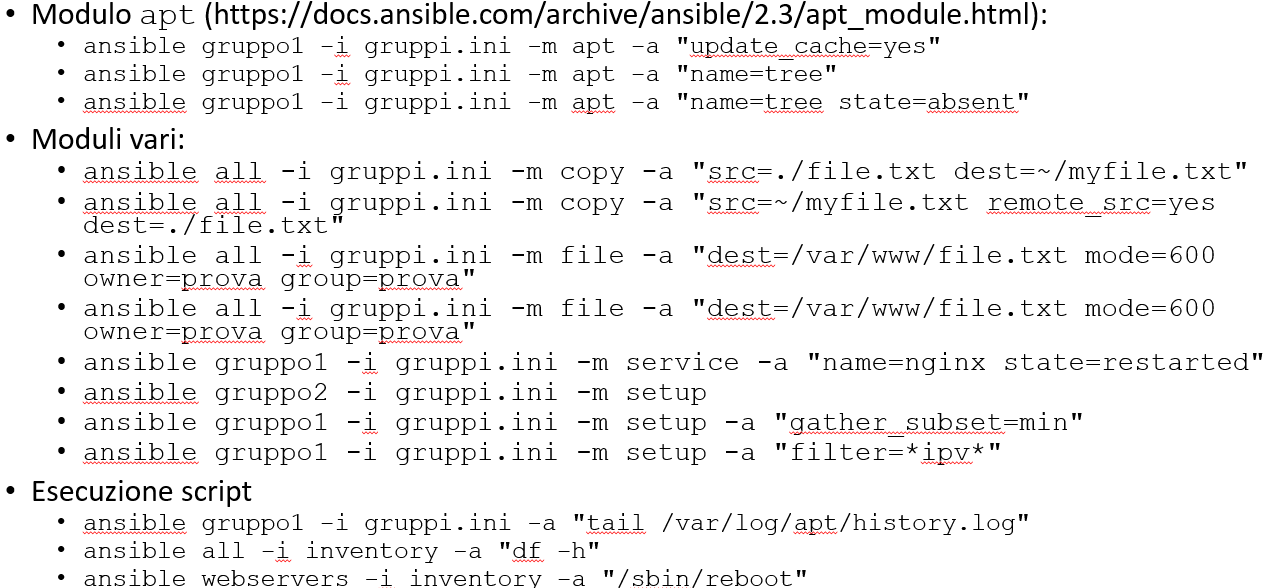
\includegraphics[keepaspectratio]{images/image2.png}}}

{}

\subsection{\texorpdfstring{{Playbook}}{Playbook}}\label{h.1mansw4tgcfr}

{Servono per eseguire comandi Ansible in modo semplice e flessibile.}

{}

{I due formati sono:}

\begin{itemize}
\tightlist
\item
  {.ini: semplici ma meno flessibili;}
\item
  {.yaml: usati praticamente sempre quando la complessità aumenta.}
\end{itemize}

{}

{Esempio di sintassi, ricordarsi che è necessario rispettare gli spazi:}

{\pandocbounded{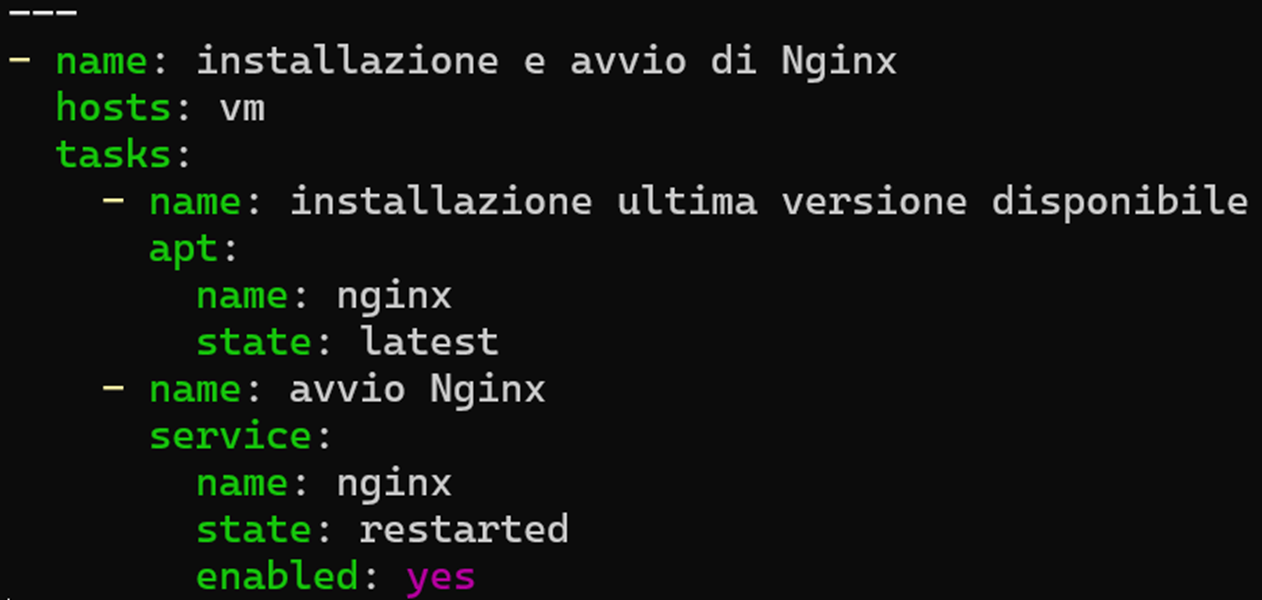
\includegraphics[keepaspectratio]{images/image4.png}}}

{Si possono avviare con il comando:}

{ansible-playbook -i inventory.ini nomeFile.yaml}

{}

{Creare un VM con docker:
}{\href{https://www.google.com/url?q=https://secgroup.dais.unive.it/teaching/vm-with-docker/&sa=D&source=editors&ust=1734629472347820&usg=AOvVaw00IuQ4t1iga6EA3ReVmFuZ}{https://secgroup.dais.unive.it/teaching/vm-with-docker/}}

{}

{Kubernetes}

{Sistema di orchestrazione di container. Composto da Nodi (macchina che
esegue attività), cluster (nodi logicamente correlati), pod (uno o più
container distribuiti su un singolo nodo, con stesso IP, IPC, nome host
ecc)) e Control plane (controlla i nodi e i cluster).}

\section{\texorpdfstring{{Set up}}{Set up}}\label{h.fmovwu69nm6c}

{Per vedere come creare e settare la macchina virtuale:
}{\href{https://www.google.com/url?q=https://unibo.cloud.panopto.eu/Panopto/Pages/Viewer.aspx?id\%3Dc51d7154-78e0-4816-a740-b22600f9d90f&sa=D&source=editors&ust=1734629472348207&usg=AOvVaw2s588O2jgrjtWScGe1O3bq}{https://unibo.cloud.panopto.eu/Panopto/Pages/Viewer.aspx?id=c51d7154-78e0-4816-a740-b22600f9d90f}}

\section{\texorpdfstring{{Comandi}}{Comandi}}\label{h.q7ah8b4ndvw9}

{Per creare un namespace:}

{kubectl create namespace nomeNamespace}

{}

{}

{Visualizzare i namespace;}

{kubectl get namespace}

{}

{}

{Creare dei deployment di un'immagine in un namespace specifico:}

{kubectl create deployment nomeDeploy --image=nomeImage
-n=nomeNamespace}

{}

{}

{Visualizzare i deployment di un namespace:}

{kubectl get deployment -n nomeNamespace}

{}

{}

{Visualizzare tutti i deployment di tutti i namespace:}

{kubectl get deployment -A}

{}

{}

{Cambiare namespace corrente:}

{kubectl config set-context - -current - -namespace=nomeNamespace}

{per assicurarsi di essere nel giusto:}

{kubectl config get-contexts}

{}

{}

{Ottenere informazioni su un deployment {[}}{DA FARE DENTRO IL
RISPETTIVO NAMESPACE}{{]}:}

{kubectl describe deployment nomeDeploy}

{}

{}

{Visualizzare il log di un deployment, utile in caso di errore {[}}{DA
FARE DENTRO IL RISPETTIVO NAMESPACE}{{]}:}

{kubectl logs deployment/nomeDeploy}

{}

{}

{Cancellare tutti i deployment di un namespace:}

{kubectl delete deployment --all -n nomeNamespace}

{}

{}

{Visualizzare in quali nodi sono in esecuzione }{i pods:}

{kubectl get pods -o wide}

{}

{MQTT}

{}

\end{document}
